%introduction-example


\usebackgroundtemplate{%             declare it
\tikz[overlay,remember picture] \node[opacity=1, at=(current page.center)] {
   \includegraphics[height=\paperheight,width=\paperwidth]{images/tradML.pdf}};
}

\begin{frame}
\end{frame}

\usebackgroundtemplate{ }
%edit as needed



\begin{frame}{Traditional Machine learning}
The older/traditional way of applying machine learning consisted of the following steps:
	\begin{enumerate}[$\bullet$]
		\item \textbf{Feature Extraction}: Features which can be used to discriminate between classes is captured. This step usually requires in-field knowledge about the problem.\pause
		\item \textbf{Model Selection}: A model is selected which trains on the extracted features. Ensable methods can be used to boost performance\pause
		\item \textbf{Cross-validation/Tested}: The model is tested/cross-validated on with held data
	\end{enumerate}
\end{frame}

\begin{frame}{Problems with the traditional approach}
	  \begin{enumerate}[$\bullet$]
		  \item \textbf{Feature Extraction}: This step requires in-field knowledge. It is very difficult to study  a whole new branch of knowledge for a single problem.\pause
		  \item \textbf{Amount of Data}: In the current era, the amount of data sometimes is simply so large that meaningful features are hard to extract \pause
		  \item \textbf{Unorganized Data}: Feature extraction is hard in unorganized data (such as a literary works).
	  \end{enumerate}
  \end{frame}

  \usebackgroundtemplate{%             declare it
  \tikz[overlay,remember picture] \node[opacity=1, at=(current page.center)] {
	 \includegraphics[height=\paperheight,width=\paperwidth]{images/idea_ddepl.pdf}};
  }

  \begin{frame}
  \end{frame}

  \usebackgroundtemplate{ }
  %edit as needed

\begin{frame}{Ideas behind a neural network}
\begin{enumerate}[$\bullet$]
	\item \textbf{Pattern recognition}: Almost all the problems with traditional Ml lies in proper feature selection. We now take a different approach: We train the machine to learn what the necessary patterns/features are.\pause
	\item \textbf{Inspiration}: For this task we take inspiration from the best pattern recognizing machine that we know:\pause\textbf{ our brains}.\pause
	\item \textbf{Overview}: We make a perceptron, which is essentially the digital analog of a neuron. We connect multiple neurons together(similar to our brain) and look at what pattern and amount of activation leads to best result.
\end{enumerate}
\end{frame}



\begin{frame}{A practical comparison with traditional ML}
	\begin{columns}[T]
	\begin{column}{0.4\textwidth}
	  \includegraphics[width=\textwidth]{images/trad vs deep.png}
	  \tiny{\textit{Comparision based on amount of data features.\\ Src: Neural Networks and Deep Learning: A Textbook, Charu C. Aggarwal}}
	\end{column}
	\begin{column}{0.6\textwidth}
	\begin{enumerate}[$\bullet$]
	\item Traditional ML models show better prediction when the amount of features involved is small. Features can be individually engineered and interpreted.\pause
	\item Deep learning models are better when data is unstructured or there are a lot of features which need to be considered. With proper construction and training almost any decision boundaries can be learned.
	\end{enumerate}
	\end{column}
  \end{columns}
\end{frame}

\usebackgroundtemplate{%             declare it
\tikz[overlay,remember picture] \node[opacity=1, at=(current page.center)] {
   \includegraphics[height=\paperheight,width=\paperwidth]{images/perceptron.pdf}};
}

\begin{frame}
\end{frame}

\usebackgroundtemplate{ }


\begin{frame}{Non-Linearity is the key}
  \begin{columns}[T]
  \begin{column}{0.4\textwidth}
	\includegraphics[width=\textwidth]{images/nobg perceptron.png}
	\tiny{\textit{A perceptron\\ Src: MIT Introduction to Deep Learning,6.S191,Lec-1}}
  \end{column}
  \begin{column}{0.6\textwidth}
  \begin{enumerate}[$\bullet$]
  \item The idea behind a perceptron is that a perceptron will give a high value as output when it recognises a certain feature.\pause
  \item Mathematically for an input vector $X$ it outputs $\hat{Y}=\sigma(W^TX+b_0)$ \pause
  \item Multiple perceptrons are wired together(again, much like our brain) to identify richer features.\pause
  \item At the very core, Machine Learning works by constructing proper decision boundaries.\pause
  \item A very simple calculation shows if $\sigma$ is linear then the decision boundary is also linear. It therefore makes sense to use non-linear $\sigma$.
  \end{enumerate}
  \end{column}
\end{columns}
\end{frame}


\begin{frame}{Non-Linearity is the key}
  \begin{columns}[T]
  \begin{column}{0.4\textwidth}
	\includegraphics[width=\textwidth]{images/non-linearity.png}
	\tiny{\textit{Non-linearity in action\\ Src: Neural Networks and Deep Learning: A Textbook, Charu C. Aggarwal}}
  \end{column}
  \begin{column}{0.6\textwidth}
  \begin{enumerate}[$\bullet$]
  \item As shown in the figure on left, classes which can't be separated by linear boundaries can be separated by non-linear functions.(Think SVM but the kernals are learned.)\pause
  \item It can be theoretically shown that almost all boundary function can be separated by a 2 layered neural network.
  \end{enumerate}
  \end{column}
\end{columns}
\end{frame}



\begin{frame}{Increasing depth}
  \begin{columns}[T]
  \begin{column}{0.4\textwidth}
	\includegraphics[width=\textwidth]{images/depth.png}
	\tiny{\textit{Why is depth needed\\ Src: Neural Networks and Deep Learning: A Textbook, Charu C. Aggarwal}}
  \end{column}
  \begin{column}{0.6\textwidth}
  \begin{enumerate}[$\bullet$]
  \item While a single hidden layer is enough, making a deep neural network allows us to have more complex decision boundaries with relatively less number of nodes\pause
  \item It should be noted how non-linearity discussed above plays an important role: Irrespective of number of layers, composition of linear functions is linear. On the other hand compositions of non-linear function can lead to richer families of functions. (\textit{Ref: https://www.desmos.com/calculator/m645ggyl2i})
  \end{enumerate}
  \end{column}
\end{columns}
\end{frame}



usebackgroundtemplate{%             declare it
\tikz[overlay,remember picture] \node[opacity=1, at=(current page.center)] {
   \includegraphics[height=\paperheight,width=\paperwidth]{images/training.pdf}};
}
\begin{frame}
\end{frame}

\usebackgroundtemplate{ }

\begin{frame}{Loss Function}
  \begin{columns}[T]
  \begin{column}{0.4\textwidth}
	\includegraphics[width=\textwidth]{images/resnet110-noskip-loss.png}
	\tiny{\textit{A slice of the loss landscape of resnet-110 with no skip connections\\ Src: Visualizing the Loss Landscape of Neural Nets, Hao Li, Zheng Xu, Gavin Taylor, Christoph Studer, Tom Goldstein}}
  \end{column}
  \begin{column}{0.6\textwidth}
  \begin{enumerate}[$\bullet$]
  \item We wish to calculate weights $w_i,1\leq i\leq n$ so that the predicted values $\hat{Y}$ are as close as possible(to an extent) to the actual values $Y$.\pause To do this we try to minimize a loss function $\mathcal{L}(\{\hat Y_i\},\{Y_i\})$\pause
  \item Common choices of $\mathcal L$ include MSE for continuous variables and cross-loss entropy for categorical variables.
  \end{enumerate}
  \end{column}
\end{columns}
\end{frame}


\begin{frame}{Gradient descent}
  \begin{columns}[T]
  \begin{column}{0.4\textwidth}
	\includegraphics[width=\textwidth]{images/grad-desc.png}
	\tiny{\textit{Gradient descent\\ Src: https://towardsdatascience.com/an-intuitive-explanation-of-gradient-descent-83adf68c9c33}}
  \end{column}
  \begin{column}{0.6\textwidth}
  \begin{enumerate}[$\bullet$]
  \item To find the correct set of weights, we use a greedy approach. We check the surrounding landscape of the weight(i.e. calculate the gradient) and take a step in the direction which leads to maximum decrease in $\mathcal L$. Mathematically, we have:
  $$w_i=wi-\eta \frac{\partial \mathcal L}{\partial w_i}$$\pause
  \item $\eta$ is known as the learning rate.
  \end{enumerate}
  \end{column}
\end{columns}
\end{frame}


\begin{frame}{Learning Rate}
  \begin{columns}[T]
  \begin{column}{0.4\textwidth}
	\includegraphics[width=1.1\textwidth]{images/learning rate.jpeg}
	\tiny{\textit{Variations in learning rates\\ Src: Hands-On Machine Learning with Scikit-Learn, Keras, and TensorFlow  Concepts, Tools, and Techniques to Build Intelligent Systems-O'Reilly Media, Inc, Aurélien Géron }}
  \end{column}
  \begin{column}{0.6\textwidth}
  \begin{enumerate}[$\bullet$]
  \item Fixing $\eta$ is quite tricky.\pause
  \item If $\eta$ is small we get stuck at local minima\pause
  \item If $\eta$ is large we overshoot our targets and never converge.
  \item The best way to do things is to use a adaptive learn rate. Some methods(parametric, non-parametric and hybrid are discussed later, once we cover backpropagation)
  \end{enumerate}
  \end{column}
\end{columns}
\end{frame}


\begin{frame}{Backpropagation}
  Consider a neural network to be an acyclic directed graph
  \begin{enumerate}[$\bullet$]
  \item We want to calculate the partial derivative of a node with respect to the other.\pause
  \item The way to do this is to use the chain rule\pause
  \item When we use the chain rule, we sum the partial derivative along all the paths joining the two nodes
  \item It is easy to see that the computation needed explodes as the depth increases
  \item The way to navigate this problem is to use dynamic programming.
  \end{enumerate}
\end{frame}

\begin{frame}
\begin{center}


\tikzset{every picture/.style={line width=0.75pt}} %set default line width to 0.75pt

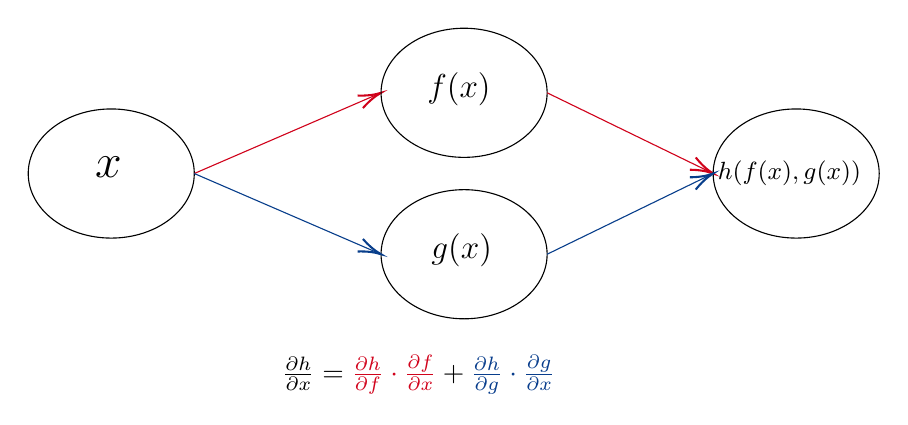
\begin{tikzpicture}[x=0.75pt,y=0.75pt,yscale=-1,xscale=1]
%uncomment if require: \path (0,300); %set diagram left start at 0, and has height of 300

%Shape: Ellipse [id:dp3367595598760599]
\draw   (0,70) .. controls (0,52.82) and (17.91,38.89) .. (40,38.89) .. controls (62.09,38.89) and (80,52.82) .. (80,70) .. controls (80,87.18) and (62.09,101.11) .. (40,101.11) .. controls (17.91,101.11) and (0,87.18) .. (0,70) -- cycle ;
%Straight Lines [id:da39910224852829135]
\draw [color={rgb, 255:red, 208; green, 2; blue, 27 }  ,draw opacity=1 ]   (80,70) -- (168.16,31.9) ;
\draw [shift={(170,31.11)}, rotate = 156.63] [color={rgb, 255:red, 208; green, 2; blue, 27 }  ,draw opacity=1 ][line width=0.75]    (10.93,-3.29) .. controls (6.95,-1.4) and (3.31,-0.3) .. (0,0) .. controls (3.31,0.3) and (6.95,1.4) .. (10.93,3.29)   ;
%Shape: Ellipse [id:dp014340350236969002]
\draw   (170,31.11) .. controls (170,13.93) and (187.91,0) .. (210,0) .. controls (232.09,0) and (250,13.93) .. (250,31.11) .. controls (250,48.29) and (232.09,62.22) .. (210,62.22) .. controls (187.91,62.22) and (170,48.29) .. (170,31.11) -- cycle ;
%Straight Lines [id:da30953970172924394]
\draw [color={rgb, 255:red, 208; green, 2; blue, 27 }  ,draw opacity=1 ]   (250,31.11) -- (328.2,69.13) ;
\draw [shift={(330,70)}, rotate = 205.92] [color={rgb, 255:red, 208; green, 2; blue, 27 }  ,draw opacity=1 ][line width=0.75]    (10.93,-3.29) .. controls (6.95,-1.4) and (3.31,-0.3) .. (0,0) .. controls (3.31,0.3) and (6.95,1.4) .. (10.93,3.29)   ;
%Shape: Ellipse [id:dp1322107562231436]
\draw   (330,70) .. controls (330,52.82) and (347.91,38.89) .. (370,38.89) .. controls (392.09,38.89) and (410,52.82) .. (410,70) .. controls (410,87.18) and (392.09,101.11) .. (370,101.11) .. controls (347.91,101.11) and (330,87.18) .. (330,70) -- cycle ;
%Shape: Ellipse [id:dp6161135526872799]
\draw   (170,108.89) .. controls (170,91.71) and (187.91,77.78) .. (210,77.78) .. controls (232.09,77.78) and (250,91.71) .. (250,108.89) .. controls (250,126.07) and (232.09,140) .. (210,140) .. controls (187.91,140) and (170,126.07) .. (170,108.89) -- cycle ;
%Straight Lines [id:da31403089636099324]
\draw [color={rgb, 255:red, 8; green, 62; blue, 139 }  ,draw opacity=1 ]   (250,108.89) -- (328.2,70.87) ;
\draw [shift={(330,70)}, rotate = 154.08] [color={rgb, 255:red, 8; green, 62; blue, 139 }  ,draw opacity=1 ][line width=0.75]    (10.93,-3.29) .. controls (6.95,-1.4) and (3.31,-0.3) .. (0,0) .. controls (3.31,0.3) and (6.95,1.4) .. (10.93,3.29)   ;
%Straight Lines [id:da9909467052529207]
\draw [color={rgb, 255:red, 8; green, 62; blue, 139 }  ,draw opacity=1 ]   (80,70) -- (168.16,108.1) ;
\draw [shift={(170,108.89)}, rotate = 203.37] [color={rgb, 255:red, 8; green, 62; blue, 139 }  ,draw opacity=1 ][line width=0.75]    (10.93,-3.29) .. controls (6.95,-1.4) and (3.31,-0.3) .. (0,0) .. controls (3.31,0.3) and (6.95,1.4) .. (10.93,3.29)   ;


% Text Node
\draw (31,60.96) node [anchor=north west][inner sep=0.75pt]  [font=\LARGE]  {$x$};
% Text Node
\draw (191,19.96) node [anchor=north west][inner sep=0.75pt]  [font=\large]  {$f( x)$};
% Text Node
\draw (193,97.73) node [anchor=north west][inner sep=0.75pt]  [font=\large]  {$g( x)$};
% Text Node
\draw (331,62.62) node [anchor=north west][inner sep=0.75pt]  [font=\small]  {$h( f( x) ,g( x))$};
% Text Node
\draw (121,156.4) node [anchor=north west][inner sep=0.75pt]    {$\frac{\partial h}{\partial x} =\textcolor[rgb]{0.82,0.01,0.11}{\frac{\partial h}{\partial f} \cdot \frac{\partial f}{\partial x}} +\textcolor[rgb]{0.03,0.24,0.55}{\frac{\partial h}{\partial g} \cdot \frac{\partial g}{\textcolor[rgb]{0.03,0.24,0.55}{\partial x}}}$};


\end{tikzpicture}

\end{center}
\end{frame}
\begin{frame}{Backpropagation}
	Roughly, the alogirithm works as follows:
	\begin{enumerate}[$\bullet$]
	\item Initialize the weights\pause
	\item Calculate $\mathcal{L}$. Note, that this step occurs from the input towards the output and is known as the forward phase.
	\item Calculate gradient. This process occurs from the output towards the input and is known as the backward phase.
	\end{enumerate}
  \end{frame}


  \begin{frame}{Reverse Mode Auto Differentiation}
	\begin{columns}[T]
	\begin{column}{0.8\textwidth}
	\begin{center}
		\includegraphics[width=\textwidth]{images/revmodeautodiff.png}
	\end{center}
	\end{column}
	\begin{column}{0.2\textwidth}
	The whole idea relies on the fact that while calculating gradients, parts of the calculation are repeated.
	\end{column}
	\end{columns}
\end{frame}

\begin{frame}{Reverse Mode Auto Differentiation}
\begin{columns}[T]
\begin{column}{0.7\textwidth}
\begin{center}
	\includegraphics[width=\textwidth]{images/path comp.png}
\end{center}
\end{column}
\begin{column}{0.3\textwidth}
Sum is taken over the product along each path, over all the paths. It is trivial to note that parts of the paths are repeated.\pause In the toy example on the left, the paths are essentially the same, varying only for the second to last node.
\end{column}
\end{columns}
\end{frame}

\begin{frame}{Gradient Descent Statergy-Stochastic Gradient Descent}
	\begin{columns}[T]
	\begin{column}{0.4\textwidth}
	  \includegraphics[width=\textwidth]{images/stochastic gradient descent.png}
	  \tiny{\textit{Stochstic Gradient descent\\ Src:Hands-On Machine Learning with Scikit-Learn, Keras, and TensorFlow  Concepts, Tools, and Techniques to Build Intelligent Systems-O'Reilly Media, Inc, Aurélien Géron}}
	\end{column}
	\begin{column}{0.6\textwidth}
	\begin{enumerate}[$\bullet$]
	\item Instead of calculating the total loss, we calculate the loss from a randomly picked sample(or a batch in case of batch gradient descent)\pause
	\item This decreases the computational time.\pause
	\item Think instead of taking slower but confident steps, we take faster but less-confident steps.
	\end{enumerate}
	\end{column}
  \end{columns}
  \end{frame}

  \begin{frame}{Gradient Descent Statergy- Normalization}
	\begin{columns}[T]
        \begin{column}{0.6\textwidth}
        	\includegraphics[width=\textwidth]{images/normalise.png}
        	\tiny{\textit{Why normalize?\\ Src:Hands-On Machine Learning with Scikit-Learn, Keras, and TensorFlow  Concepts, Tools, and Techniques to Build Intelligent Systems-O'Reilly Media, Inc, Aurélien Géron}}
        \end{column}
	    \begin{column}{0.4\textwidth}
    	    Normalizing features is a way to make the descent smoother. It essentially lowers the changes in direction orthogonal to the minima.
    	\end{column}
    \end{columns}
\end{frame}


  \begin{frame}{Gradient Descent Statergy- Mommentum}
    \begin{columns}[T]
    \begin{column}{0.4\textwidth}
      \includegraphics[width=\textwidth]{images/momentum.png}
      \tiny{\textit{Need for momentum\\ Src:Neural Networks and Deep Learning: A Textbook, Charu C. Aggarwal}}
    \end{column}
    \begin{column}{0.6\textwidth}
    \begin{enumerate}[$\bullet$]
    \item A Momentum term might be used in gradient descent where consideration is made for a moving average "velocity" of the descent.\pause
    \item Particularly helps when there are local minimas and flat regions. \pause
    \item  Helps when there is a lot of "zig-zag" but the descent heads in a certain direction.
    \end{enumerate}
    \end{column}
    \end{columns}
\end{frame}


\begin{frame}{Gradient Descent Statergy- Mommentum}
  \begin{columns}[T]
    \begin{column}{0.4\textwidth}
		\includegraphics[width=\textwidth]{images/momentum-zigzag.png}
        \tiny{\textit{Need for momentum\\ Src:Neural Networks and Deep Learning: A Textbook, Charu C. Aggarwal}}
    \end{column}
    \begin{column}{0.6\textwidth}
    \begin{enumerate}[$\bullet$]
      \item A Momentum term might be used in gradient descent where consideration is made for a moving average "velocity" of the descent.
      \item Particularly helps when there are local minimas and flat regions.
      \item  Helps when there is a lot of "zig-zag" but the descent heads in a certain direction.
      \end{enumerate}
      \end{column}
      \end{columns}
      \end{frame}

\begin{frame}{Gradient Descent Statergy- Nestov Mommentum}
	\begin{columns}[T]
        \begin{column}{0.4\textwidth}
        	\includegraphics[width=\textwidth]{images/nestov.png}
        	\tiny{\textit{Nestov momentum\\ Src:Hands-On Machine Learning with Scikit-Learn, Keras, and TensorFlow  Concepts, Tools, and Techniques to Build Intelligent Systems-O'Reilly Media, Inc, Aurélien Géron}}
        \end{column}
	    \begin{column}{0.6\textwidth}
    	    \begin{enumerate}[$\bullet$]
        		\item Nestov-momentum is similar to momentum with some scout ahead\pause
        		\item Knowing what's coming up ahead further helps in correcting the direction of descent.
        	\end{enumerate}
    	\end{column}
    \end{columns}
\end{frame}

\begin{frame}{Gradient Descent Statergy- Adaptive Learning Rates}
    \begin{enumerate}[$\bullet$]
		\item We try to let different parameters have different learning rates.\pause
		\item The idea is that parameters with large partial derivatives are often oscillating and
		zigzagging, whereas parameters with small partial derivatives tend to be more consistent
		but move in the same direction.\pause
		\item  Algorithms include AdaGrad, RMSProp and AdaDelta. Parametric algorithms combined with momentum considerations also exist: RMSProp with Nesterov Momentum, ADAM and it's variants like AdaMax, Nadam and AdamW. A quick comparison table is avilable at \textit{Hands-On Machine Learning with Scikit-Learn, Keras, and TensorFlow  Concepts, Tools, and Techniques to Build Intelligent Systems-O'Reilly Media, Inc by Aurélien Géron}
    \end{enumerate}
\end{frame}



\begin{frame}{Gradient Descent Statergy- Learning Rate Scheduling}
	\begin{columns}[T]
        \begin{column}{0.4\textwidth}
        	\includegraphics[width=\textwidth]{images/learning rate schedule.png}
        	\tiny{\textit{Nestov momentum\\ Src:Hands-On Machine Learning with Scikit-Learn, Keras, and TensorFlow  Concepts, Tools, and Techniques to Build Intelligent Systems-O'Reilly Media, Inc, Aurélien Géron}}
        \end{column}
	    \begin{column}{0.6\textwidth}
    	    \begin{enumerate}[$\bullet$]
        		\item We have the learning rate high at first so that it gets a relative idea about where the minima lies\pause, and then we lower it to find it with more accuracy\pause
        		\item Scheduling is done on numbers of iterations completed(each iteration is also called an \textit{epoch})\pause
        	\end{enumerate}
    	\end{column}
    \end{columns}
\end{frame}


\begin{frame}{Gradient Descent Statergy- One cycle scheduling}
    \begin{enumerate}[$\bullet$]
		\item The basic idea behind one cycle scheduling is to start with a low learning rate, gradually increase it to a maximum value, and then decrease it again to a low value. This approach helps the network explore a wide range of learning rates, allowing it to quickly converge to a good solution and potentially escape from local minima.
		\item By using a cyclical learning rate schedule, one cycle scheduling aims to strike a balance between exploration and exploitation in the learning process. It enables the network to quickly explore a wide range of learning rates at the beginning and then gradually refine its weights as the learning rate decreases.
    \end{enumerate}
\end{frame}

\begin{frame}{Gradient Descent Strategy- Choosing an activation function}
	\begin{columns}[T]
        \begin{column}{0.5\textwidth}
        	\includegraphics[width=\textwidth]{images/sgn.png}
        	\tiny{\textit{$sgn(x)$}}
        \end{column}
	    \begin{column}{0.5\textwidth}
    	    One of the first activation functions to be considered was $sgn(x)$ mostly because this was the function based on which our neurons operate.
    	\end{column}
    \end{columns}
\end{frame}

\begin{frame}{Gradient Descent Strategy- Choosing an activation function}
	\begin{columns}[T]
        \begin{column}{0.5\textwidth}
        	\includegraphics[width=\textwidth]{images/sigmoid.png}
        	\tiny{\textit{$sigmoid$}}
        \end{column}
	    \begin{column}{0.5\textwidth}
    	    But soon better activation functions were found like the \textcolor{red}{sigmoid} function
    	\end{column}
    \end{columns}
\end{frame}

\begin{frame}{Gradient Descent Strategy- Choosing an activation function}
	\begin{columns}[T]
        \begin{column}{0.5\textwidth}
        	\includegraphics[width=\textwidth]{images/tanh.png}
        	\tiny{\textit{$sigmoid$,$tanh$}}
        \end{column}
	    \begin{column}{0.5\textwidth}
    	    But soon better activation functions were found like the \textcolor{red}{sigmoid} function, \textcolor{green}{tanh} function
    	\end{column}
    \end{columns}
\end{frame}

\begin{frame}{Gradient Descent Strategy- Choosing an activation function}
	\begin{columns}[T]
        \begin{column}{0.5\textwidth}
        	\includegraphics[width=\textwidth]{images/relu.png}
        	\tiny{\textit{$sigmoid$,$tanh$,$relu$}}
        \end{column}
	    \begin{column}{0.5\textwidth}
    	    But soon better activation functions were found like the \textcolor{red}{sigmoid} function, \textcolor{green}{tanh} function and \textcolor{blue}{relu} function.
    	\end{column}
    \end{columns}
\end{frame}

\begin{frame}{Gradient Descent Strategy- Dead Neurons and Vanishing \& Exploding Gradients}
	\begin{columns}[T]
        \begin{column}{0.5\textwidth}
        	\includegraphics[width=\textwidth]{images/relu.png}
        	\tiny{\textit{$sigmoid$,$tanh$,$relu$}}
        \end{column}
	    \begin{column}{0.5\textwidth}
    	    \begin{enumerate}[$\bullet$]
				\item Most activation function saturated. Therefore, high values meant no gradient "propagated" forward. This leads to neurons which rarely activated and became "dead".\pause 
				\item The effect of derivatives magnifies down the layers. If the order of magnitude is above 1(say $10$) then it explodes(after 10 layers it will become $10^{10}$).
			\end{enumerate}
    	\end{column}
    \end{columns}
\end{frame}

\begin{frame}{Gradient Descent Strategy- Dead Neurons and Vanishing \& Exploding Gradients}
	\begin{columns}[T]
        \begin{column}{0.5\textwidth}
        	\includegraphics[width=\textwidth]{images/relu.png}
        	\tiny{\textit{$sigmoid$,$tanh$,$relu$}}
        \end{column}
	    \begin{column}{0.5\textwidth}
    	    \begin{enumerate}[$\bullet$]
				\item The effect of derivatives magnifies down the layers. If the order of magnitude is below 1(say $1/10$) then it vanishes(after 10 layers it will become $10^{-10}$)\pause
				\item From a more practical viewpoint, this might lead to overflow if the gradient explodes. If it is vanishing, then there might not be enough precision to handle the values.
			\end{enumerate}
    	\end{column}
    \end{columns}
\end{frame}

\begin{frame}{Gradient Descent Strategy- Better Activation Functions}
	\begin{columns}[T]
        \begin{column}{0.5\textwidth}
        	\includegraphics[width=\textwidth]{images/LeakyRelu.png}
        	\tiny{\textit{$leaky$ $ReLu$}}
        \end{column}
	    \begin{column}{0.5\textwidth}
    	    One way to alleviate those problems is to use better activation function which are in a way variants of ReLu. Some examples include 
			\begin{enumerate}[$\bullet$]
				\item \textcolor{blue}{Leaky ReLu $\left(\max(\alpha z,z)\right)$}
			\end{enumerate}
    	\end{column}
    \end{columns}
\end{frame}



\begin{frame}{Gradient Descent Strategy- Better Activation Functions}
	\begin{columns}[T]
        \begin{column}{0.5\textwidth}
        	\includegraphics[width=\textwidth]{images/ELU.png}
        	\tiny{\textit{$leaky$ $ReLu$, $ELU$}}
        \end{column}
	    \begin{column}{0.5\textwidth}
    	    One way to alleviate those problems is to use better activation function which are in a way variants of ReLu. Some examples include 
			\begin{enumerate}[$\bullet$]
				\item \textcolor{blue}{Leaky ReLu $\left(\max(\alpha z,z)\right)$}
				\item \textcolor{red}{ELU$\left((\alpha (e^z-1)\text{if $z<0$ else }z)\right)$} 
			\end{enumerate}
    	\end{column}
    \end{columns}
\end{frame}

\begin{frame}{Gradient Descent Strategy- Better Activation Functions}
	\begin{columns}[T]
        \begin{column}{0.5\textwidth}
        	\includegraphics[width=\textwidth]{images/SELU.png}
        	\tiny{\textit{$leaky$ $ReLu$, $ELU$, $SELU$}}
        \end{column}
	    \begin{column}{0.5\textwidth}
    	    One way to alleviate those problems is to use better activation function which are in a way variants of ReLu. Some examples include 
			\begin{enumerate}[$\bullet$]
				\item \textcolor{blue}{Leaky ReLu $\left(\max(\alpha z,z)\right)$}
				\item \textcolor{red}{ELU$\left((\alpha (e^z-1)\text{if $z<0$ else }z)\right)$} 
				\item \textcolor{green}{SELU$\left(1.05ELU_{1.67}\right)$}
			\end{enumerate}
    	\end{column}
    \end{columns}
\end{frame}

\begin{frame}{Gradient Descent Strategy- Better Activation Functions}
	\begin{columns}[T]
        \begin{column}{0.5\textwidth}
        	\includegraphics[width=\textwidth]{images/SELU.png}
        	\tiny{\textit{$leaky$ $ReLu$, $ELU$, $SELU$}}
        \end{column}
	    \begin{column}{0.5\textwidth}
    	    One way to alleviate those problems is to use better activation function which are in a way variants of ReLu. Some examples include 
			\begin{enumerate}[$\bullet$]
				\item \textcolor{blue}{Leaky ReLu $\left(\max(\alpha z,z)\right)$}
				\item \textcolor{red}{ELU$\left((\alpha (e^z-1)\text{if $z<0$ else }z)\right)$} 
				\item \textcolor{green}{SELU$\left(1.05ELU_{1.67}\right)$}
			\end{enumerate}
			One can also treat $\alpha$ as a parameter to be learned by back prop. 
    	\end{column}
    \end{columns}
\end{frame}

\begin{frame}{Gradient Descent Strategy- Better Activation Functions}
	\begin{columns}[T]
        \begin{column}{0.5\textwidth}
        	\includegraphics[width=\textwidth]{images/GELU.png}
        \end{column}
	    \begin{column}{0.5\textwidth}
    	    Other activation functions also exists such as 
			\begin{enumerate}[$\bullet$]
				\item \textcolor{blue}{GELU $\left(z\Phi(z)\right)$}where $\Phi$ is the CDF of the standard normal
			\end{enumerate}
    	\end{column}
    \end{columns}
\end{frame}

\begin{frame}{Gradient Descent Strategy- Better Activation Functions}
	\begin{columns}[T]
        \begin{column}{0.5\textwidth}
        	\includegraphics[width=\textwidth]{images/SWISH.png}
        \end{column}
	    \begin{column}{0.5\textwidth}
    	    Other activation functions also exists such as 
			\begin{enumerate}[$\bullet$]
				\item \textcolor{blue}{GELU $\left(z\Phi(z)\right)$}where $\Phi$ is the CDF of the standard normal.
				\item \textcolor{red}{SWISH $\left(z\sigma(z)\right)$}where $\sigma$ is the sigmoid function.
			\end{enumerate}
    	\end{column}
    \end{columns}
\end{frame}

\begin{frame}{Gradient Descent Strategy- Better Activation Functions}
	\begin{columns}[T]
        \begin{column}{0.5\textwidth}
        	\includegraphics[width=\textwidth]{images/MISH.png}
        \end{column}
	    \begin{column}{0.5\textwidth}
    	    Other activation functions also exists such as 
			\begin{enumerate}[$\bullet$]
				\item \textcolor{blue}{GELU $\left(z\Phi(z)\right)$}where $\Phi$ is the CDF of the standard normal.
				\item \textcolor{red}{SWISH $\left(z\sigma(z)\right)$}where $\sigma$ is the sigmoid function.
				\item \textcolor{green}{MISH $\left(z\tanh(\ln(1+exp(z)))\right)$}where $\sigma$ is the sigmoid function.
			\end{enumerate}
    	\end{column}
    \end{columns}
\end{frame}

\begin{frame}{Gradient Descent Strategy- Weight Initialization}
	\begin{enumerate}[$\bullet$]
		\item Initially weights were initialized by picking from a standard normal distribution.\pause
		\item The difference in the variance of the outgoing nodes and incoming nodes(if there is a difference in number of nodes between layers) cause practical problems in the flow of gradients.\pause
		\item A good compromise is to take average of number of outgoing edges and number of incoming edges and normalize the variance of the normal distribution used by it. This is called Glorot initialization\pause The same principal when used with uniform distribution is called He initialization.
	\end{enumerate}
\end{frame}

\begin{frame}{Gradient Descent Strategy- Gradient Clipping}
	\begin{enumerate}[$\bullet$]
		\item In case one of the components of the gradient is much lager than other we might want to normalize it to control our descent.\pause
		\item One way it to just limit it at some maximum value.\pause
		\item Other methods include normalizing the whole vector with respect to a norm. 
	\end{enumerate}
\end{frame}

\begin{frame}{Aspects of a deep neural network-navigating the loss landscape}
	\begin{enumerate}[$\bullet$]
		\item Generally, as far as decision boundaries are concerned, adding depth gives ore bang for the buck than adding more nodes in a single layer.\pause But depth comes with its own share of problems.\pause
		\item Deeper networks have a harder time converging.\pause
		\item If activation functions are not combined properly then there might be presence of local minimas
	\end{enumerate}
\end{frame}
\begin{frame}{Aspects of a deep neural network-skip connections}
	\begin{columns}[T]
        \begin{column}{0.4\textwidth}
        	\includegraphics[width=\textwidth]{images/skip.png}
			\tiny{\textit{Skip connections\\ Src:Neural Networks and Deep Learning: A Textbook, Charu C. Aggarwal}}
        \end{column}
	    \begin{column}{0.6\textwidth} 
			\begin{enumerate}[$\bullet$]
				\item We might allow nodes from deeper layers to have direct access to nodes from shallower layers while \textit{skipping} the intermediate layers.\pause
				\item This provides a kind of highway for the deeper layers to access simpler features.\pause
				\item This is especially used in CNNs.
			\end{enumerate}
    	\end{column}
    \end{columns}
\end{frame}
\begin{frame}{Aspects of a deep neural network-maxout networks }
	\begin{columns}[T]
        \begin{column}{0.4\textwidth}
        	\includegraphics[width=\textwidth]{images/maxout.png}
			\tiny{\textit{Max-out connections\\ Src:Improving deep neural networks with multilayer maxout networks, Weichen Sun, Fei Su, Leiquan Wang}}
        \end{column}
	    \begin{column}{0.6\textwidth} 
			\begin{enumerate}[$\bullet$]
				\item In a certain sense this is type of ensemble method.\pause
				\item Two sets of weights $W_1,W_2$ are trained for each input.
				\item The activation is set to $\sigma\left(\max(W_1\cdot X_{in},W_2\cdot X_{in})+b_0\right)$
			\end{enumerate}
    	\end{column}
    \end{columns}
\end{frame}

\begin{frame}{Aspects of a deep neural network-navigating the loss landscape}
	\begin{enumerate}[$\bullet$]
		\item Generally, as far as decision boundaries are concerned, adding depth gives ore bang for the buck than adding more nodes in a single layer.\pause But depth comes with its own share of problems.\pause
		\item Deeper networks have a harder time converging.\pause
		\item If activation functions are not combined properly then there might be presence of local minimas
	\end{enumerate}
\end{frame}
